\documentclass[10pt,pdf,utf8,aspectratio=169,xcolor=dvipsnames,x11names,center]{beamer}

\usepackage[T2A]{fontenc}
\usepackage[english,russian]{babel}
\usepackage[utf8]{inputenc}

\usepackage{pgfpages}
%%\setbeameroption{show notes}
%%\setbeameroption{show notes on second screen=right}

\usepackage{dirtytalk}

\usepackage{listings}

\definecolor{light-gray}{gray}{0.95}
\lstset{
language=Python,                             % Code langugage
basicstyle=\small,                   % Code font, Examples: \footnotesize, \ttfamily
keywordstyle=\color{OliveGreen},        % Keywords font ('*' = uppercase)
commentstyle=\color{gray},              % Comments font
numbers=left,                           % Line nums position
numberstyle=\tiny,                      % Line-numbers fonts
stepnumber=1,                           % Step between two line-numbers
numbersep=5pt,                          % How far are line-numbers from code
backgroundcolor=\color{light-gray},     % Choose background color
frame=lines,                            % A frame around the code
tabsize=4,                              % Default tab size
captionpos=b,                           % Caption-position = bottom
breaklines=true,                        % Automatic line breaking?
breakatwhitespace=false,                % Automatic breaks only at whitespace?
showspaces=false,                       % Don't make spaces visible
showstringspaces=false,                 % Don't show spaces in string literals 
showtabs=false,                         % Don't make tabs visible
}

\title[Remote]{\Large{Про то, как\\эффективно работать\\в распределенной команде,\\но может и нет}}

\author[]{\Large{Стас Рудаков}\\\small{stas@garage22.net}}

\date{Minsk Python Meetup\\December 2017}

\begin{document}

\begin{frame}
  \titlepage

  \note{
    Вообще говоря, я планировал прочитать этот доклад на январском
    митапе. Все дело в том, что мне через неделю исполняется 30 лет. То
    есть я стою на пороге кризиса среднего возраста. Мне казалось
    важным войти в этот период переод прочтением доклада. С одной
    стороны, смотрю я на свои достижения к 30 годам, и, как любой
    честный перед собой человек, понимаю, что особо ничего я не
    добился. С другой стороны, страсть как хочется свой опыт кому-то
    передать. Итак, меня зовут Стас Рудаков, мне без недели 30 лет, я
    ничего особенного в жизни не сделал, и теперь научу вам, как я
    этого добился.
  }

\end{frame}

\begin{frame}
  \begin{figure}
    \includegraphics[scale=0.05]{DataRobot_Logo}
  \end{figure}

  \note{
    Собственно, два года назад я начал сотрудничать с компанией
    DataRobot, при этом большую часть времени работая удаленно. Мне в
    какой-то мере повезло: DataRobot уже имел значительный для стартапа
    опыт с распределенными командами. Поэтому мне не пришлось
    выстраивать процессы с нуля. Скорее пришлось интегрироваться в уже
    неплохо работающие подходы. О том, что работало, а что нет, я и
    хочу сегодня рассказать.
  }

\end{frame}

\begin{frame}
  \frametitle{Беспочвенное утверждение 1}

  \note {
    Но для начала я бы хотел заявить что-то, не приводя никаких
    серьезных аргументов.
  }

  \pause Технологии и рынок труда меняются так быстро, что\\
  любой переход на позицию, не требующую ежедневной работы с кодом,\\
  ухудшает карьерные перспективы для разработчика в Беларуси.

  \vspace{0.6cm} \pause Но это не значит, что вы не должны быть
  способны перейти на такую позицию.

  \note{
    Пока что мы работает с кодом, мы наиболее мобильны. В ситуации,
    когда все меняется так стремительно, мобильность --- очень важное
    свойство. Она позволяет нам критически относиться к тому, чем мы
    занимаемся, а также быть максимально мотивированными и
    продуктвными.
  }

\end{frame}

\begin{frame}
  \frametitle{Основные вызовы в распределенных командах}
  \centering
  
  \begin{minipage}{9cm}
    Для индивида
    \pause
    \begin{itemize}
    \item Самомотивация
    \item Нехватка общения
    \item Стирается граница личное-рабочее
    \item Мультипликация проблем
    \end{itemize}
  \end{minipage}

  \note {
    Но давайте поговорим, какие вызовы стоят перед индивидумами,
    работающими в распределенных командах. Во-первых, по умолчанию
    система не подталкивает вас. Так или иначе, нужно думать, как
    подталкивать себя самому. Плюс в силу нехватки общения, любая
    проблема может вырасти до крупной значительно быстрее, чем при
    работе с локальной командой.
  }
  
  \vspace{0.6cm}
  \pause

  \begin{minipage}{9cm}
    Для команды
    \pause
    \begin{itemize}
    \item Эффективная коммуникация
    \item Культурные различия
    \item Часовые пояса
    \item Эффективное стимулирование членов команды
    \item Установление доверительных отношений между членами команды
    \end{itemize}
  \end{minipage}

  \note {
    Для команды вызовы тоже значительные. Для локальных команд
    накоплен большой опыт, как вести себя в тех или иных
    ситуациях. Например, вывез команду в ресторан после крупного
    успеха --- это одновременно и стимулирует, и помогает установить
    доверительные отношения. В распределенной команде же нужно гораздо
    больше изобретать.
  }
  
\end{frame}

\begin{frame}
  \frametitle{Технологический сдвиг}

  \begin{itemize}
  \item Collaborative Documents: G Suite, Office365
  \item Github / Gitlab / Bitbucket
  \item Чаты: Slack, HipChat
  \item Видео-конференции: Hangouts, Zoom, Slack
  \item Больше облаков: Jira, Confluence, Trello, Яндекс.Коннект
  \item CI: Travis, Codeship, Circle
  \item Инфраструктура: AWS, Google Cloud, Digital Ocean
  \item Real time collaboration: Teletype for Atom, \ldots
  \end{itemize}

  \note {
    Но на самом деле инструменты для совместной работы двигаются
    вперед так быстро, что граница между распределенными и
    нераспределенными командами размывается. Этому, конечно,
    способствует повсеместное принятие облачных сервисов. Еще 5 лет
    назад было тяжело себе представить, что средние и крупные
    компании доверят свою рабочую почту облачным провайдерам. Ведь
    вне защищенной корпоративной сети нельзя говорить ни о какой
    защите информации. Сегодня же мне даже тяжело придумать
    аргументы, почему новые компании могут хотеть хостить почту на
    своем железе.
  }

  \note {
    Получается, что если команда позволяет своим сотрудникам время от
    времени работать из дому, эта команда становится в какой-то мере
    распределенной. И вызовы, встающие перед ней, все те же.
  }

  \note {
    Вообще забавно, как новые инструменты, с одной стороны, дают
    свободу индивидам, а с другой --- эту же свободы
    забирают. Например, условный Slack позволяет не привязываться к
    физической локации и все еще быть вовлеченным во внутренние
    процессы. Но с другой стороны, это порождает always-on проблемы,
    когда по сути сотрудник остается на рабочем месте круглые
    сутки. И чтобы эту проблему преодолеть, нередко нужно проявить
    силу воли, расставить приоритеты.
  }
\end{frame}

\begin{frame}
  \frametitle{Беспочвенное утверждение 2}

  \note{Я планирую продолжить серию своих ничем не обоснованных утверждений.}
  
  \pause Разработчику нет смысла не становиться более эффективным.

  \note{
    Конечно, от повышения моей эффективности выигрывает
    работодатель. Но делаю я это в первую очередь для себя. Сегодня
    профессия открывает перед нами широкие горизонты. И работа над
    собственной эффективностью нужна не кому-то, а в первую очередь
    нам с вами.
  }

  \note{
    Вообще говоря, не профессия такая, а время такое. Раньше как
    было: вот тебе буржуа, владеющий средствами производства, вот
    тебе пролетарий, непосредственно работающий. Все просто и
    понятно. Но сегодня все мы с вами одновременно и буржуа, и
    пролетарии. Поэтому от того, что наш внутренний пролетарий
    становится более эффективным, выигрывает в первую очередь наш
    внутренний буржуа.
  }
\end{frame}

\begin{frame}
  \frametitle{Самоуправление}

  \begin{itemize}
  \item Планируйте свое время
  \item Ставьте себе цели
  \item Делайте отчеты о своей работе
  \item Будьте прозрачны
  \item Отвечайте за свою карьеру
  \end{itemize}

  \note{
    Забавно, что все эти советы не имеют ничего общего именно с
    распределенными командами. Вопрос лишь в том, что для локальных
    команд легче иметь специально обученный менеджмент, который будет
    приглядывать за этими вопросами. Вас легче расспросить на кухне,
    вас легче ``прочитать'' по невербальным признакам в случае
    локальной команды. Но строго говоря, это просто базовые навыки
    опытного специалиста.
  }
\end{frame}

\begin{frame}
  \frametitle{Беспочвенное утверждение 3}

  \note{Надеюсь, вы уже заждались моих ничем необоснованных заявлений.}
  

  \note{
    Когда я только начинал свою карьеру, для меня сложным вопросом
    было, должен ли я ставить во главу угла свои личные интересы,
    интересы своих коллег или интересы компании.
  }

  \note{
    Это, как мне кажется, очень советское наследие окопалось в моей
    голове, когда все эти интересы разведены по разным углам.
  }

  \note{
    Сегодня ответ для меня очевиден. Вопрос: должен ли я ставить во
    главу угла свои личные интересы, интересы своих коллег или
    интересы компании? Ответ: да.
  }

  \note{
    Просто потому что, в условиях сегодняшнего рынка глупо разделять
    все эти успехи. В западных странах для придания выгодного стимула
    давно разработали вполне работающие механизмы: та же раздача
    долей компании сотрудникам в виде опционов.
  }

  \note{
    Тем не менее, даже в Беларуси вариантов продолжения карьеры у нас
    огромное множество. Выбирать те, где интересы личные, интересы
    команды и интересы компании конфликтуют, чаще всего
    нерационально.
  }

  \note{
    Поэтому хочу подчеркнуть свою позицию: нет смысла работать без
    цели добиться успеха. При этом сегодня становится очень сложным
    добиваться чего-либо значительно в одиночку. Гораздо эффективнее
    действовать командами или компаниями. Поэтому я лично
    заинтересован в том, чтобы мои команада и компания были в как
    можно более здоровом состоянии.
  }

  \pause Нет смысла работать без цели добиться успеха.
\end{frame}

\begin{frame}
  \frametitle{Коммуникация I}

  \begin{itemize}
  \item Коммуникация асинхронна по умолчанию
  \item Нужны четкие точки входа
    \begin{itemize}[<.(1)->]
    \item Куда писать email, чтобы его прочитала вся команда?
    \item Куда пойти, чтобы пообщаться с командой в чате?
    \item Как понять, какая команда отвечает за ту или иную подсистему?
    \item Как просить PR review у команды, которая отвечает за эту область кода?
    \end{itemize}
  \item Нужно прояснить, как эскалировать вопрос, если методы выше не работают
  \item Нужно прояснить временные зоны, в которые есть смысл ожидать ответа
  \end{itemize}

  \note{
    Итак, в распределенной команде коммуникация асинхронна по
    умолчанию. Очень важны точки входа: должны быть механизмы общения
    с командой и они должны работать. Где и как мне пообщаться с
    командой? В какое время суток мне ожидать ответ? Кому
    эскалировать вопрос, если я не получаю ответа? Через какое время
    после задания вопроса стоит эскалировать? Ясность по этим
    вопросам значительно упрощает жизнь всем.
  }

\end{frame}

\begin{frame}
  \frametitle{Коммуникация II}

  \begin{itemize}
  \item Все члены команды следят за эффективной коммункацией
    \begin{itemize}[<.(1)->]
    \item Если есть возможность/знания, дают ответы на запросы
    \item Если нет возможности/знаний, пытаются привлечь нужных людей
    \end{itemize}
  \item Худшее при коммуникации --- молчание на другой стороне
  \item Если есть проблемы с поддержанием коммуникации, нужно определять ключевые индикаторы и цели
  \end{itemize}

  \note{
    Запросы, приходящие к команде изнутри и извне, не должны
    оставаться без внимания. Очень важно не хранить молчание:
    * Если даже у вас нет конкретного ответа, вы можете как минимум знать, у
      кого этот ответ есть.
    * Если у всей команды нет конкретного ответа, дайте знать, что вы
      работаете над тем, чтобы разузнать детали, обозначьте сроки.
    * Если сейчас есть более приоритетная работа, не держите это в тайне.
      Снова таки, обозначьте сроки.
    * Хочу акцентировать внимание: я не пытаюсь сказать, что все члены команды
      должны незамедлительно отвечать на вопросы в Slack. Например, вам может
      понадобиться 4 часа сфокусированного времени - и это нормально.
      Просто дайте знать об этом вашим коллегам.
  }
\end{frame}

\begin{frame}
  \frametitle{Коммуникация III: Документ vs Дискуссия}

  \begin{itemize}
  \item Дискуссия хорошо подходит, если идея не сформирована
  \item Документы (спецификации, предложения) хорошо подходят, если идея уже сформирована, но вам нужно услышать чужое мнение
    \begin{itemize}[<.(1)->]
    \item Написать документ дешевле, чем написать код
    \item Написанный документ можно переиспользовать
    \item Асинхронная коммуникация
    \end{itemize}
  \item Даже если вы не хотите слышать ничье мнение, все равно опишите свою идею
  \end{itemize}
  
\end{frame}

\begin{frame}
  \frametitle{Коммуникация IV: Code Review}

  \note{
    Мы разработчики, поэтому общаться кодом для нас часто привычнее
    всего. Давайте на примере процесса PR review посмотрим на
    какие-то маленькие трюки. Но для начала хочу заметить, что, как и
    многое другое, о чем я сегодня говорю, code review --- это не
    цель, а средство или инструмент. В зависимости от особенностей
    вашей организации детали использования этого инструмента,
    конечно, могут быть другими. Поэтому я обозначю из каких целей я
    буду исходить далее.
  }

  \pause

  \begin{minipage}{9cm}
    Цели
    \begin{itemize}
    \item Общее владение кодом
    \item Коммуникация об изменениях
    \item Поддержание ожидаемого уровня качества кода
    \item Обучение коллег, выработка единого стиля
    \item Быстрые итерации
    \end{itemize}
  \end{minipage}

  \vspace{0.6cm}

  \begin{minipage}{9cm}
    Не-цели
    \begin{itemize}
    \item Повышение самооценки
    \item Уберегание драгоценного репозитория от плохих изменений
    \end{itemize}
  \end{minipage}

\end{frame}

\begin{frame}
  \begin{figure}
    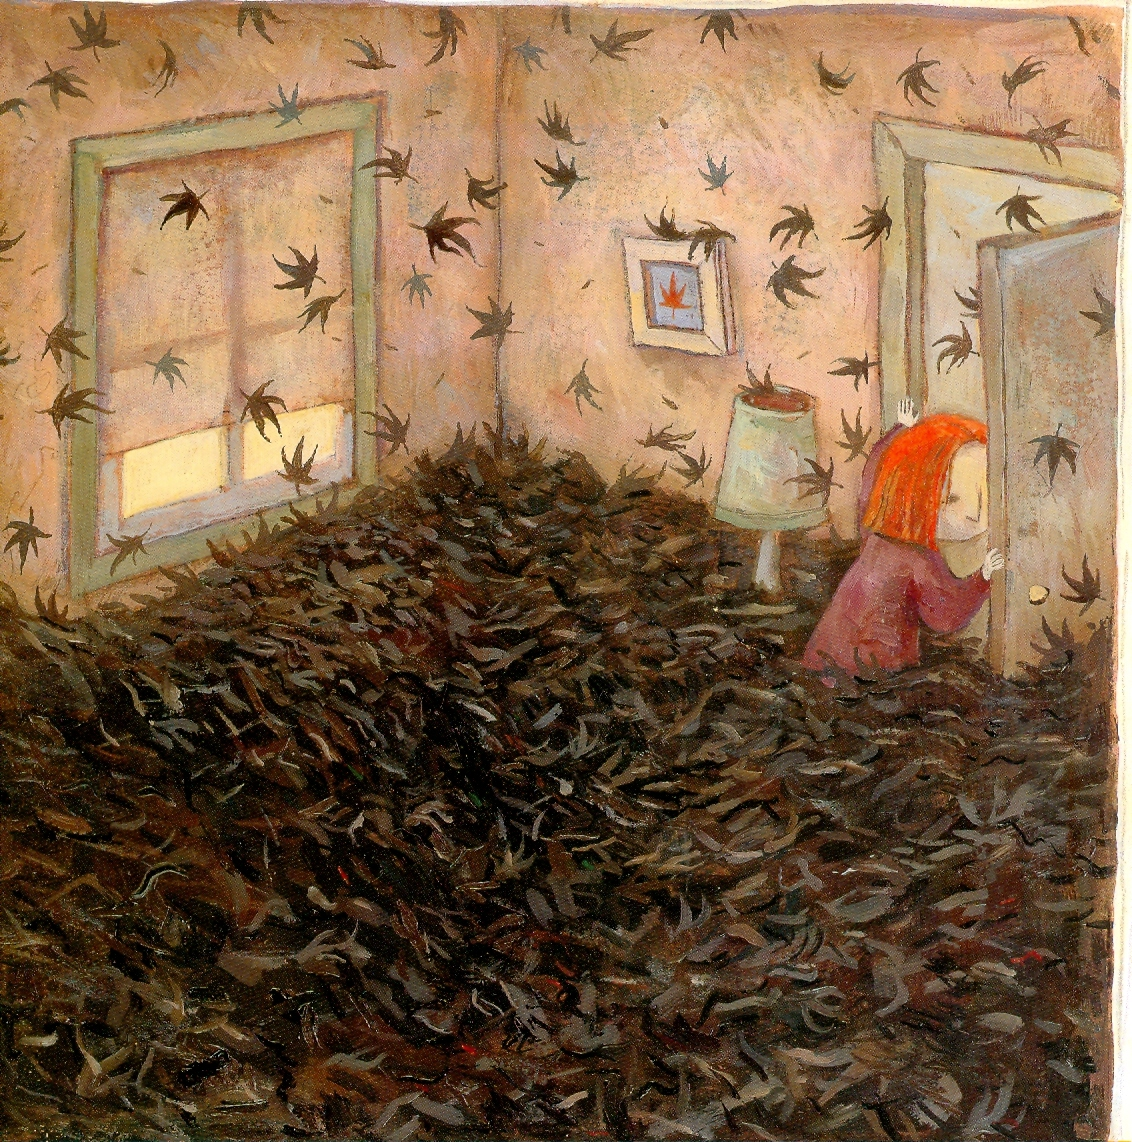
\includegraphics[scale=0.6]{redtree}
  \end{figure}
\end{frame}

\begin{frame}[fragile]
  \frametitle{Code Review: Opinion vs Facts}
  \begin{lstlisting}[caption=D]
    def do_something(strange, really):
  \end{lstlisting}

  \begin{lstlisting}[caption=D]
    def do_something(
        strange, really
    ):
  \end{lstlisting}

  \begin{lstlisting}[caption=D]
    def do_something(strange,
                     really):
  \end{lstlisting}

  \begin{lstlisting}[caption=D]
    def do_something(
        strange, really):
  \end{lstlisting}

\end{frame}

\begin{frame}[fragile]
  \frametitle{Code Review: Ad-Hoc Requests}

  \say{Кстати, раз уж ты правишь код, не мог бы ты исправить еще \ldots и \ldots}
  \pause
  \vspace{0.6cm}

  \say{Нет!}
  \pause
  \vspace{0.6cm}

  Просто создавайте тикеты.

\end{frame}

\begin{frame}[fragile]
  \frametitle{Code Review: вместо тысячи слов...}

  \say{Мне кажется, эту функцию можно переписать так, чтобы внутренний цикл \ldots,\\а потом использовать паттерн \ldots}
  \pause
  \vspace{0.6cm}

  \begin{lstlisting}
    for i in range(0, len(items), batch_size):
        ...
        items[i:i+batch_size]
  \end{lstlisting}

\end{frame}

\begin{frame}
  \frametitle{Brian Anderson: советы}

  \url{http://brson.github.io/2017/04/05/minimally-nice-maintainer}
  \begin{itemize}
  \item Отвечайте быстро
  \item Говорите ``спасибо''
  \item Хвалите
  \item Говорите ``Да''
  \item Устанавливайте четкие ожидания
  \item Признавайте ошибки
  \item Будьте эмоциональны
  \end{itemize}

  \note{
    Полгода назад я прочитал блог пост от Brian Anderson, в котором
    он описывает, каким должен быть maintainer open source проекта. В
    тот момент Brian был лидером проекта Rust. Если вы не следите за
    этим языком, то я лишь добавлю, что они умудряются двигаться
    вперед очень быстро, оставаяюсь при этом действительно
    прозрачными. С точки зрения процесса разработки команда языка
    Rust действительно большие молодцы.
  }

  \note{
    Так вот, этот блог пост срезонировал со мной. Поэтому я попытаюсь
    проиллюстрировать, как эти же идеи можно легко и эффективно
    переложить на процесс code review.
  }

  \note{
    Забавный факт: через несколько месяцев после написания этого
    поста Brian добровольно покинул пост лидера языка. В тексте, в
    котором он мотивировал это решение, четко прослеживался факт
    профессионального выгорания. Для меня это еще раз подтверждает тот факт,
    что без правильного режима отдыха невозможно быть эффективным на
    долгой дистанции.
  }
\end{frame}

\begin{frame}
  \begin{figure}
    
\includegraphics[scale=0.5]{approve}
  \end{figure}
\end{frame}

\begin{frame}
    \begin{block}{Стас Рудаков}
    \par \url{mailto:stas@garage22.net}
    \par \url{http://staaas.net/talks.html}
    \end{block}
\end{frame}

\end{document}
